%% Material suplementar do artigo SERRA (soja, Oeste do Paraná).
%% As tabelas vêm de tabelas_suplementares.tex, gerado por ../analise/06_suplementar.py -- não editar à mão.
%% Compilar: latexmk -pdf supplementary.tex
\documentclass[11pt,a4paper]{article}
\usepackage[margin=2.2cm]{geometry}
\usepackage{graphicx}
\usepackage{booktabs}
\usepackage{longtable}
\usepackage{float}
\usepackage{amsmath,amssymb}
\usepackage{xcolor}
\usepackage[hidelinks]{hyperref}

\newcommand{\inserir}[1]{\textcolor{red}{[INSERIR #1]}}
\renewcommand{\thetable}{S\arabic{table}}
\renewcommand{\thefigure}{S\arabic{figure}}
\renewcommand{\thesection}{S\arabic{section}}

\title{Supplementary material for\\ ``Season-blocked validation, error structure and shortfall risk of soybean yield forecasts from satellite and reanalysis data in western Paraná, Brazil''}
\author{Julia Tluszcz, Pedro Luiz de Paula Filho, Fabrício Correia de Oliveira}
\date{}

\begin{document}
\maketitle
\tableofcontents

%% GERADO por analise/06_suplementar.py a partir de resultados/ -- não editar à mão

\section{Predictors}

\begin{table}[H]
\centering
\caption{Predictors of the municipality--season dataset (93 in total). Phase predictors were computed for each of the four phases.}\label{tab:S_pred}
\small
\begin{tabular}{@{}llll@{}}
\toprule
Predictor & Unit & Source & Phases \\
\midrule
Precipitation & mm & CHIRPS & F1--F4 \\
Days with $P < 1$ mm & days & CHIRPS & F1--F4 \\
Potential evapotranspiration & mm & ERA5-Land & F1--F4 \\
Actual evapotranspiration & mm & ERA5-Land & F1--F4 \\
Water balance $P - ET_p$ (Eq. 1) & mm & CHIRPS, ERA5-Land & F1--F4 \\
Days with $T_{max} > 32\,^\circ$C & days & ERA5-Land & F1--F4 \\
Mean air temperature & $^\circ$C & ERA5-Land & F1--F4 \\
Mean maximum air temperature & $^\circ$C & ERA5-Land & F1--F4 \\
Mean minimum air temperature & $^\circ$C & ERA5-Land & F1--F4 \\
Absolute maximum air temperature & $^\circ$C & ERA5-Land & F1--F4 \\
Mean dew-point temperature & $^\circ$C & ERA5-Land & F1--F4 \\
Mean soil temperature, 0--7 cm & $^\circ$C & ERA5-Land & F1--F4 \\
Volumetric soil water, 0--7 cm & m$^3$ m$^{-3}$ & ERA5-Land & F1--F4 \\
Volumetric soil water, 7--28 cm & m$^3$ m$^{-3}$ & ERA5-Land & F1--F4 \\
Global solar radiation & MJ m$^{-2}$ & ERA5-Land & F1--F4 \\
Net solar radiation & MJ m$^{-2}$ & ERA5-Land & F1--F4 \\
Leaf area index of low vegetation & -- & ERA5-Land & F1--F4 \\
Maximum NDVI & -- & MOD13Q1, MYD13Q1 & F1--F4 \\
Mean NDVI & -- & MOD13Q1, MYD13Q1 & F1--F4 \\
Maximum EVI & -- & MOD13Q1, MYD13Q1 & F1--F4 \\
Mean EVI & -- & MOD13Q1, MYD13Q1 & F1--F4 \\
Seasonal maximum NDVI and EVI & -- & MOD13Q1, MYD13Q1 & season \\
Number of valid vegetation observations & -- & MOD13Q1, MYD13Q1 & season \\
Soybean area & ha & MapBiomas Collection 10 & season \\
Clay and sand content & \% & Tluszcz (2025) & static \\
Latitude, longitude, altitude & $^\circ$, m & IBGE & static \\
\bottomrule
\end{tabular}
\end{table}


\section{Validation results}

\begingroup\footnotesize
\begin{longtable}{@{}lllrrrrr@{}}
\caption{Test performance of all datasets, validation schemes and models (MAE and RMSE in kg ha$^{-1}$).}\label{tab:S_cv}\\
\toprule
Dataset & Scheme & Model & $R^2$ & MAE & RMSE & $R^2_{anom}$ & Skill \\
\midrule
\endfirsthead
\toprule
Dataset & Scheme & Model & $R^2$ & MAE & RMSE & $R^2_{anom}$ & Skill \\
\midrule
\endhead
Earlier (replica) & Random & Trend & 0.15 & 517 & 687 & 0.00 & 0.00 \\
Earlier (replica) & Random & LightGBM & 0.80 & 236 & 330 & 0.77 & 0.77 \\
Earlier, misaligned & Random & Trend & 0.15 & 518 & 685 & 0.00 & 0.00 \\
Earlier, misaligned & LOSO & Trend & $-$0.03 & 565 & 755 & 0.00 & 0.00 \\
Earlier, misaligned & Random & LightGBM & 0.81 & 237 & 326 & 0.77 & 0.77 \\
Earlier, misaligned & LOSO & LightGBM & $-$0.39 & 622 & 877 & $-$0.35 & $-$0.35 \\
Earlier, aligned & Random & Trend & 0.15 & 507 & 679 & 0.00 & 0.00 \\
Earlier, aligned & LOSO & Trend & $-$0.02 & 554 & 747 & 0.00 & 0.00 \\
Earlier, aligned & Random & LightGBM & 0.81 & 226 & 317 & 0.78 & 0.78 \\
Earlier, aligned & LOSO & LightGBM & 0.25 & 477 & 640 & 0.27 & 0.27 \\
New & Random & Trend & 0.16 & 502 & 671 & 0.00 & 0.00 \\
New & Random & Ridge & 0.79 & 249 & 333 & 0.75 & 0.75 \\
New & Random & Random forest & 0.83 & 221 & 305 & 0.79 & 0.79 \\
New & Random & XGBoost & 0.82 & 227 & 313 & 0.78 & 0.78 \\
New & Random & LightGBM & 0.83 & 216 & 300 & 0.80 & 0.80 \\
New & LOSO & Trend & 0.02 & 547 & 735 & 0.00 & 0.00 \\
New & LOSO & Ridge & 0.59 & 361 & 475 & 0.58 & 0.58 \\
New & LOSO & Random forest & 0.45 & 411 & 550 & 0.44 & 0.44 \\
New & LOSO & XGBoost & 0.47 & 403 & 539 & 0.46 & 0.46 \\
New & LOSO & LightGBM & 0.47 & 404 & 541 & 0.46 & 0.46 \\
New & Rolling & Trend & $-$0.20 & 665 & 868 & $-$0.01 & 0.00 \\
New & Rolling & Ridge & 0.37 & 500 & 627 & 0.47 & 0.48 \\
New & Rolling & Random forest & 0.22 & 544 & 699 & 0.34 & 0.35 \\
New & Rolling & XGBoost & 0.31 & 522 & 658 & 0.42 & 0.43 \\
New & Rolling & LightGBM & 0.27 & 524 & 675 & 0.39 & 0.40 \\
New & Mun. out & Trend & 0.60 & 338 & 468 & 0.00 & 0.00 \\
New & Mun. out & LightGBM & 0.79 & 245 & 337 & 0.48 & 0.48 \\
New, + Landsat & LOSO & LightGBM & 0.47 & 402 & 538 & 0.46 & 0.46 \\
\bottomrule
\end{longtable}
\endgroup


\section{Model and trend comparisons}

\begin{table}[H]
\centering
\caption{Differences in mean squared error between models under LOSO, with 95\% intervals from 2000 bootstrap replicates of whole seasons.}\label{tab:S_boot}
\small
\begin{tabular}{@{}lrcr@{}}
\toprule
Comparison (A $-$ B) & $\Delta$MSE ($10^3$ kg$^2$ ha$^{-2}$) & 95\% interval & Replicates $\ge 0$ \\
\midrule
Ridge - trend & $-$314.6 & [$-$658.5; $-$95.4] & 0.000 \\
Ridge - RF & $-$77.4 & [$-$166.4; 9.1] & 0.043 \\
Ridge - XGB & $-$64.6 & [$-$140.8; 12.6] & 0.050 \\
Ridge - LGB & $-$67.6 & [$-$145.5; 10.7] & 0.051 \\
LGB fusion - LGB MODIS only & $-$3.6 & [$-$17.2; 8.6] & 0.302 \\
\bottomrule
\end{tabular}
\end{table}
\begin{table}[H]
\centering
\caption{Effect of the form of the technological trend under LOSO (MAE in kg ha$^{-1}$).}\label{tab:S_trend}
\small
\begin{tabular}{@{}llrrr@{}}
\toprule
Trend & Model & $R^2$ & MAE & Skill \\
\midrule
Linear, municipal & Trend & 0.02 & 547 & 0.000 \\
Linear, municipal & Ridge & 0.59 & 361 & 0.583 \\
Quadratic, municipal & Trend & $-$0.04 & 567 & 0.000 \\
Quadratic, municipal & Ridge & 0.56 & 375 & 0.577 \\
Linear, regional slope & Trend & 0.00 & 549 & 0.000 \\
Linear, regional slope & Ridge & 0.60 & 363 & 0.596 \\
\bottomrule
\end{tabular}
\end{table}


\section{Performance by municipality}

\begingroup\footnotesize
\begin{longtable}{@{}llrrrrr@{}}
\caption{LOSO performance of ridge regression by municipality (MAE and RMSE in kg ha$^{-1}$; AUC for shortfall below 80\% of the trend, blank when no shortfall occurred).}\label{tab:S_mun}\\
\toprule
Municipality & Microregion & MAE & RMSE & Skill & $r$ anomaly & AUC shortfall \\
\midrule
\endfirsthead
\toprule
Municipality & Microregion & MAE & RMSE & Skill & $r$ anomaly & AUC shortfall \\
\midrule
\endhead
Anahy & Cascavel & 236 & 281 & 0.65 & 0.85 & 1.00 \\
Boa Vista da Aparecida & Cascavel & 270 & 363 & 0.49 & 0.74 & 1.00 \\
Braganey & Cascavel & 246 & 326 & 0.35 & 0.74 & 1.00 \\
Cafelândia & Cascavel & 306 & 395 & 0.65 & 0.82 & 1.00 \\
Campo Bonito & Cascavel & 293 & 400 & 0.35 & 0.65 & 0.96 \\
Capitão Leônidas Marques & Cascavel & 406 & 556 & $-$0.07 & 0.48 & 0.95 \\
Cascavel & Cascavel & 245 & 302 & 0.44 & 0.71 & 0.83 \\
Catanduvas & Cascavel & 277 & 392 & $-$0.15 & 0.41 & 0.92 \\
Corbélia & Cascavel & 292 & 414 & 0.12 & 0.58 & 0.96 \\
Diamante do Sul & Cascavel & 367 & 433 & 0.28 & 0.57 & 1.00 \\
Guaraniaçu & Cascavel & 377 & 480 & $-$0.52 & 0.34 & 0.96 \\
Ibema & Cascavel & 323 & 428 & $-$0.09 & 0.48 & 0.83 \\
Iguatu & Cascavel & 260 & 410 & $-$0.63 & 0.56 & 0.96 \\
Lindoeste & Cascavel & 321 & 414 & 0.06 & 0.56 & 0.98 \\
Nova Aurora & Cascavel & 292 & 389 & 0.73 & 0.86 & 0.87 \\
Santa Lúcia & Cascavel & 432 & 582 & $-$0.85 & 0.24 & 0.91 \\
Santa Tereza do Oeste & Cascavel & 282 & 377 & 0.04 & 0.57 &  \\
Três Barras do Paraná & Cascavel & 348 & 470 & 0.10 & 0.51 & 0.96 \\
Céu Azul & Foz do Iguaçu & 279 & 371 & 0.69 & 0.84 & 1.00 \\
Foz do Iguaçu & Foz do Iguaçu & 525 & 706 & 0.39 & 0.63 & 0.86 \\
Itaipulândia & Foz do Iguaçu & 367 & 501 & 0.68 & 0.83 & 0.95 \\
Matelândia & Foz do Iguaçu & 402 & 496 & 0.65 & 0.81 & 0.97 \\
Medianeira & Foz do Iguaçu & 440 & 545 & 0.65 & 0.83 & 1.00 \\
Missal & Foz do Iguaçu & 437 & 579 & 0.63 & 0.80 & 0.95 \\
Ramilândia & Foz do Iguaçu & 327 & 426 & 0.69 & 0.84 & 0.97 \\
Santa Terezinha de Itaipu & Foz do Iguaçu & 387 & 532 & 0.55 & 0.75 & 0.92 \\
Serranópolis do Iguaçu & Foz do Iguaçu & 436 & 561 & 0.64 & 0.80 & 0.96 \\
São Miguel do Iguaçu & Foz do Iguaçu & 395 & 544 & 0.68 & 0.83 & 0.96 \\
Vera Cruz do Oeste & Foz do Iguaçu & 366 & 456 & 0.65 & 0.81 & 0.95 \\
Assis Chateaubriand & Toledo & 309 & 394 & 0.81 & 0.91 & 0.96 \\
Diamante D'Oeste & Toledo & 372 & 478 & 0.54 & 0.74 & 0.93 \\
Entre Rios do Oeste & Toledo & 432 & 526 & 0.65 & 0.84 & 0.95 \\
Formosa do Oeste & Toledo & 424 & 717 & $-$0.36 & 0.38 & 0.82 \\
Guaíra & Toledo & 373 & 485 & 0.64 & 0.81 & 0.96 \\
Iracema do Oeste & Toledo & 370 & 432 & 0.75 & 0.87 & 0.96 \\
Jesuítas & Toledo & 322 & 373 & 0.79 & 0.89 & 0.96 \\
Marechal Cândido Rondon & Toledo & 387 & 461 & 0.72 & 0.86 & 0.96 \\
Maripá & Toledo & 380 & 493 & 0.71 & 0.85 & 0.93 \\
Mercedes & Toledo & 392 & 484 & 0.65 & 0.81 & 0.95 \\
Nova Santa Rosa & Toledo & 495 & 611 & 0.62 & 0.80 & 0.95 \\
Ouro Verde do Oeste & Toledo & 304 & 385 & 0.79 & 0.93 & 1.00 \\
Palotina & Toledo & 410 & 525 & 0.69 & 0.83 & 0.93 \\
Pato Bragado & Toledo & 453 & 533 & 0.65 & 0.85 & 0.98 \\
Quatro Pontes & Toledo & 476 & 555 & 0.60 & 0.78 & 0.90 \\
Santa Helena & Toledo & 408 & 508 & 0.64 & 0.81 & 0.94 \\
São José das Palmeiras & Toledo & 462 & 537 & 0.66 & 0.86 & 0.94 \\
São Pedro do Iguaçu & Toledo & 271 & 351 & 0.71 & 0.85 & 1.00 \\
Toledo & Toledo & 365 & 457 & 0.70 & 0.87 & 0.97 \\
Tupãssi & Toledo & 338 & 390 & 0.76 & 0.89 & 0.94 \\
\bottomrule
\end{longtable}
\endgroup


\section{Results by season}

\begingroup\footnotesize
\begin{longtable}{@{}rrrrrrrrr@{}}
\caption{Regional mean yield (kg ha$^{-1}$), Moran's $I$ of the LOSO residuals and coverage (\%) of the municipal 90\% intervals by season.}\label{tab:S_safra}\\
\toprule
Season & Observed & Forecast & Trend & Moran's $I$ & $p$ & Conformal & Mixed & CQR \\
\midrule
\endfirsthead
\toprule
Season & Observed & Forecast & Trend & Moran's $I$ & $p$ & Conformal & Mixed & CQR \\
\midrule
\endhead
2001 & 3239 & 3189 & 2763 & 0.02 & 0.248 & 96 & 98 & 98 \\
2002 & 3118 & 2982 & 2815 & 0.26 & 0.001 & 100 & 100 & 100 \\
2003 & 3134 & 3292 & 2841 & 0.21 & 0.001 & 98 & 98 & 98 \\
2004 & 2386 & 2876 & 2953 & 0.71 & 0.001 & 71 & 76 & 53 \\
2005 & 2623 & 2722 & 2944 & 0.08 & 0.086 & 98 & 98 & 92 \\
2006 & 2239 & 2487 & 2994 & 0.31 & 0.002 & 84 & 84 & 63 \\
2007 & 3070 & 3199 & 2947 & 0.21 & 0.004 & 100 & 100 & 100 \\
2008 & 3271 & 3063 & 2957 & 0.26 & 0.002 & 100 & 100 & 100 \\
2009 & 2182 & 2450 & 3041 & 0.22 & 0.002 & 76 & 76 & 88 \\
2010 & 3319 & 3308 & 3001 & 0.40 & 0.001 & 100 & 100 & 100 \\
2011 & 3428 & 3506 & 3019 & 0.31 & 0.002 & 100 & 100 & 100 \\
2012 & 1931 & 2443 & 3104 & 0.34 & 0.001 & 71 & 71 & 55 \\
2013 & 3553 & 3511 & 3057 & 0.42 & 0.001 & 100 & 100 & 100 \\
2014 & 3437 & 3165 & 3082 & 0.31 & 0.001 & 98 & 98 & 98 \\
2015 & 3365 & 3576 & 3106 & 0.55 & 0.001 & 98 & 98 & 100 \\
2016 & 3473 & 3642 & 3121 & 0.00 & 0.356 & 100 & 100 & 100 \\
2017 & 3735 & 3489 & 3126 & 0.46 & 0.001 & 96 & 98 & 96 \\
2018 & 3596 & 3262 & 3151 & 0.25 & 0.002 & 90 & 90 & 94 \\
2019 & 2694 & 2788 & 3234 & 0.18 & 0.010 & 96 & 96 & 100 \\
2020 & 3947 & 3320 & 3157 & 0.39 & 0.001 & 61 & 63 & 69 \\
2021 & 3413 & 4138 & 3221 & 0.55 & 0.001 & 49 & 53 & 96 \\
2022 & 1634 & 1571 & 3443 & 0.26 & 0.001 & 80 & 80 & 47 \\
2023 & 3279 & 3113 & 3278 & 0.27 & 0.001 & 92 & 92 & 96 \\
2024 & 3243 & 3257 & 3307 & 0.33 & 0.001 & 100 & 100 & 100 \\
2025 & 3610 & 3202 & 3267 & 0.47 & 0.001 & 82 & 82 & 94 \\
\bottomrule
\end{longtable}
\endgroup


\section{Shortfall risk}

\begin{table}[H]
\centering
\caption{Skill of shortfall probability forecasts by threshold (\% of the trend).}\label{tab:S_risk}
\small
\begin{tabular}{@{}lrrrrr@{}}
\toprule
Threshold & Frequency & Brier & Brier clim. & BSS & AUC \\
\midrule
< 70\% & 0.117 & 0.058 & 0.107 & 0.46 & 0.96 \\
< 80\% & 0.164 & 0.070 & 0.144 & 0.51 & 0.94 \\
< 90\% & 0.243 & 0.094 & 0.194 & 0.52 & 0.92 \\
\bottomrule
\end{tabular}
\end{table}
\begin{table}[H]
\centering
\caption{Reliability of shortfall probability forecasts: bins of forecast probability.}\label{tab:S_rel}
\small
\begin{tabular}{@{}lrrr@{}}
\toprule
Threshold & Mean forecast probability & Observed frequency & Forecasts \\
\midrule
< 70\% & 0.03 & 0.03 & 1072 \\
< 70\% & 0.29 & 0.62 & 80 \\
< 70\% & 0.49 & 0.85 & 20 \\
< 70\% & 0.72 & 0.46 & 13 \\
< 70\% & 0.96 & 0.88 & 40 \\
< 80\% & 0.06 & 0.03 & 938 \\
< 80\% & 0.29 & 0.28 & 112 \\
< 80\% & 0.50 & 0.78 & 73 \\
< 80\% & 0.67 & 0.82 & 44 \\
< 80\% & 0.95 & 0.79 & 58 \\
< 90\% & 0.09 & 0.02 & 651 \\
< 90\% & 0.28 & 0.21 & 259 \\
< 90\% & 0.49 & 0.45 & 93 \\
< 90\% & 0.71 & 0.83 & 106 \\
< 90\% & 0.92 & 0.86 & 116 \\
\bottomrule
\end{tabular}
\end{table}



\section{Spatial dependence of the residuals}

\begin{figure}[ht]
\centering
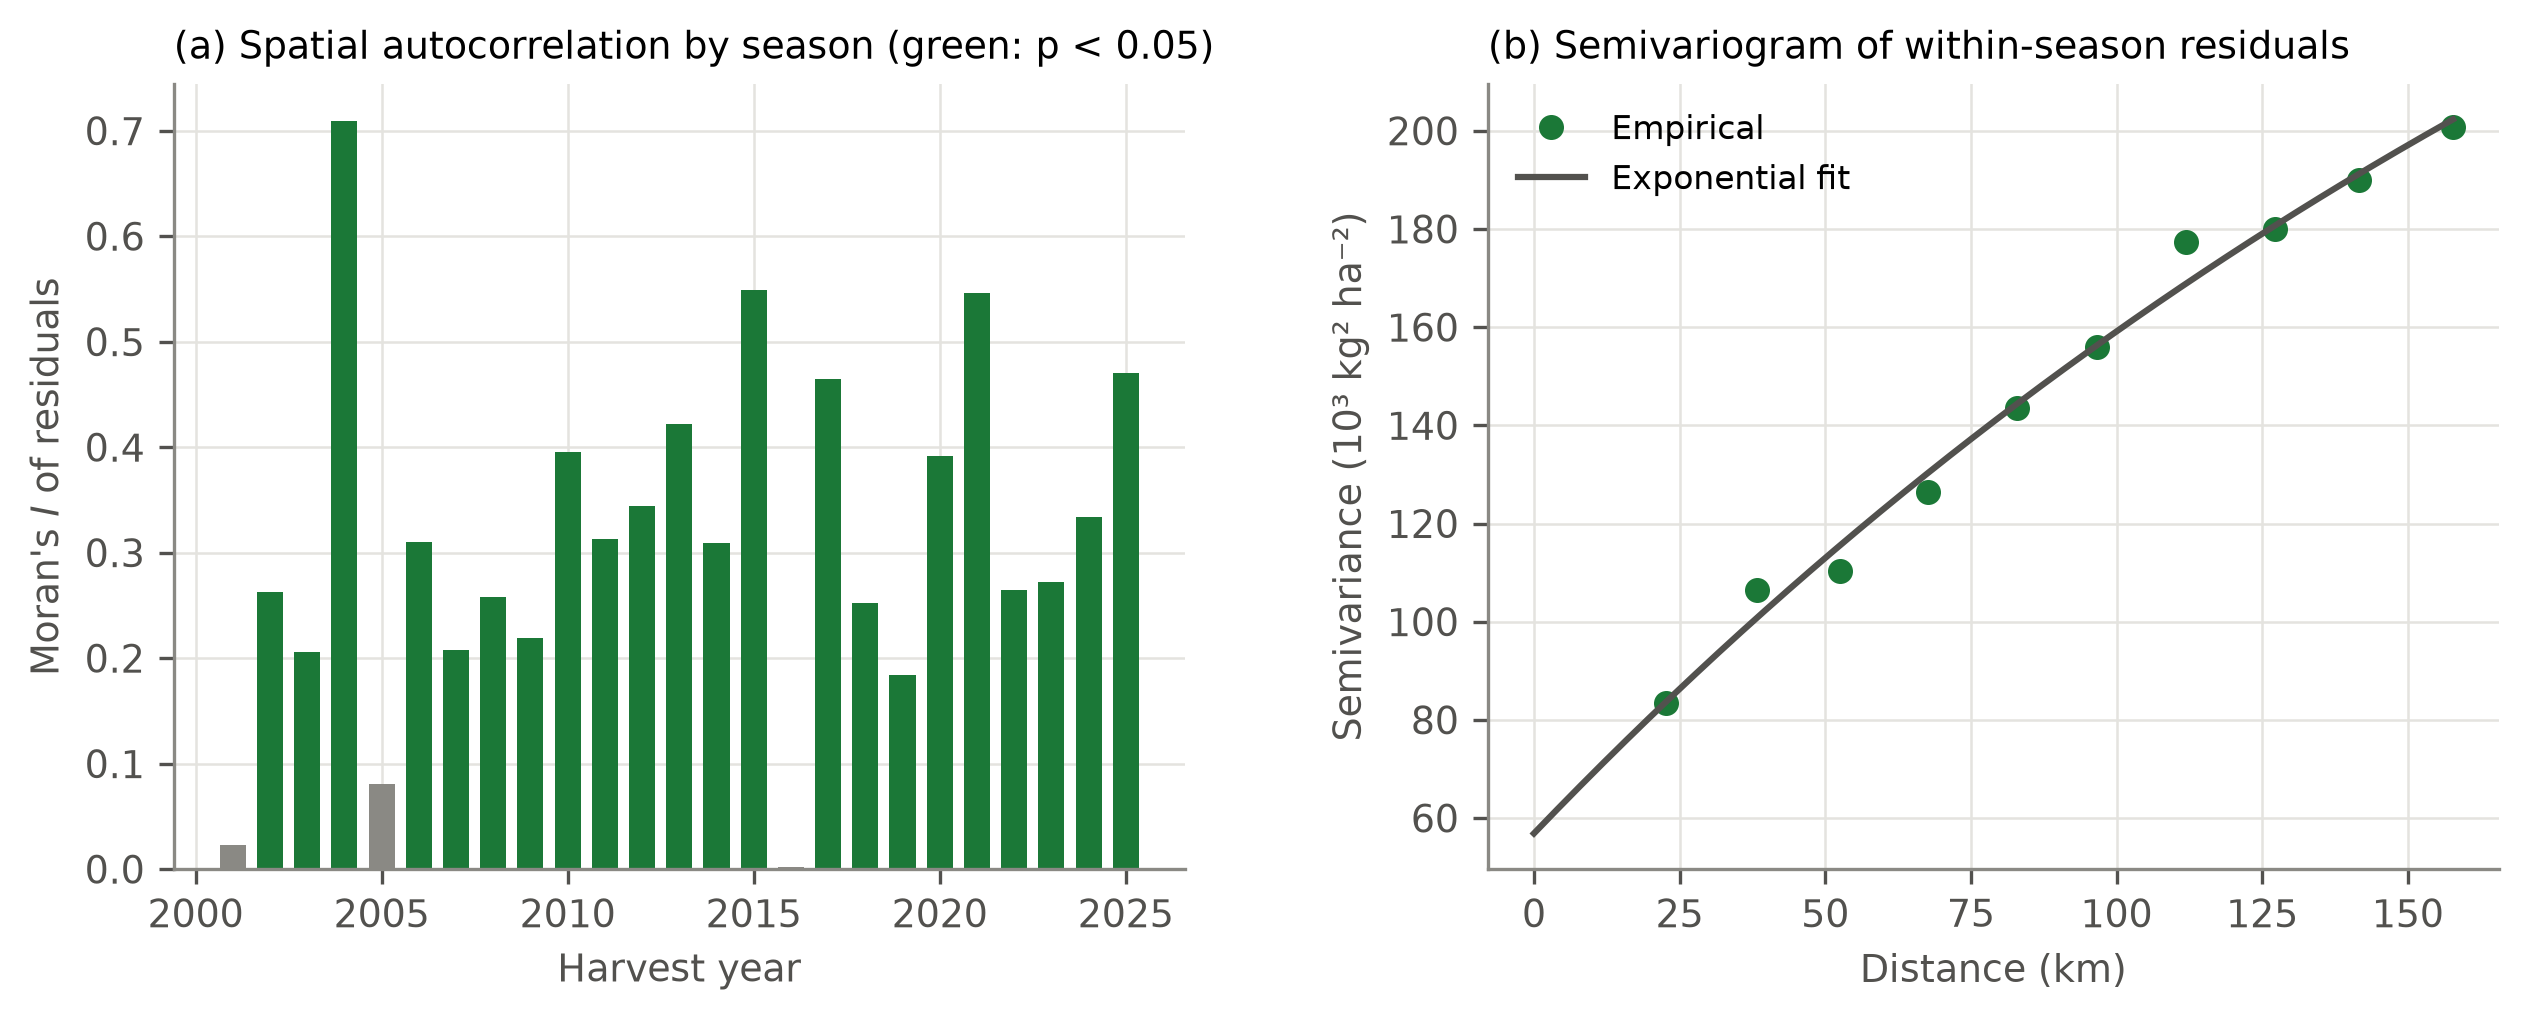
\includegraphics[width=\textwidth]{figuras/figS1_moran_variograma.png}
\caption{(a) Moran's $I$ of the LOSO residuals of ridge regression by season, with six-nearest-neighbour weights and 999 permutations; (b) empirical semivariogram of the within-season residuals pooled over seasons, in 15-km distance classes with at least 20 pairs, and fitted exponential model.}
\label{fig:S_moran}
\end{figure}

\end{document}
